
%(BEGIN_QUESTION)
% Copyright 2012, Tony R. Kuphaldt, released under the Creative Commons Attribution License (v 1.0)
% This means you may do almost anything with this work of mine, so long as you give me proper credit

Each of the electric-driven pumps in this distillation process is backed up by a redundant steam-driven pump, automatically started by a system using redundant pressure switches to sense low discharge pressure from the electric pump:

$$\includegraphics[width=15.5cm]{i0001rx01.eps}$$

Suppose PSL-62 has a PFD value of 0.0051 and PSL-63 has a PFD value of 0.0048.  Calculate the {\it dependability} of these two redundant pressure switches (i.e. the probability that together they will provide the necessary signal(s) to the auto-start system of pump P-13 if the discharge pressure falls below their trip points).

\vskip 20pt \vbox{\hrule \hbox{\strut \vrule{} {\bf Suggestions for Socratic discussion} \vrule} \hrule}

\begin{itemize}
\item{} A very helpful problem-solving technique when working with probabilities is to {\it sketch a logic function diagram} with each line in that diagram labeled with an easy-to-understand description of its real-life meaning.  Sketch such a diagram for this problem, and then explain how that diagram is helpful.
\item{} What other component or susbsystem PFD values would need to be considered in order to calculate the reliability of the entire auto-start system for pump P-13?
\item{} What are the pressure relief valves at the top of the main fractionation tower set to different ``lift'' pressures?
\end{itemize}

\underbar{file i02036}
%(END_QUESTION)





%(BEGIN_ANSWER)

Note: pay attention to Note 1 in the P\&ID!!

%(END_ANSWER)





%(BEGIN_NOTES)

According to Note 1 in the P\&ID, this is a 2oo2 trip system: {\it both} pressure switches must trip in order to start pump P-13.  This means the dependability of the two switches taken together is less than the dependability of either switch on its own.

\vskip 10pt

PFD$_{PSL-62}$ = 0.0051 \hskip 20pt $R_{PSL-62}$ = 0.9949

\vskip 10pt

PFD$_{PSL-63}$ = 0.0048 \hskip 20pt $R_{PSL-63}$ = 0.9952

\vskip 10pt

Since both switch PSL-62 {\it ans} PSL-63 must successfully trip on demand, the dependability for both in this 2oo2 system is an ``AND'' function (the mathematical product) of their individual dependabilities:

\vskip 10pt

$(R_{PSL-62})(R_{PSL-63}) = (0.9949)(0.9952) = 0.99012448$ 











\vskip 20pt \vbox{\hrule \hbox{\strut \vrule{} {\bf Virtual Trip-testing} \vrule} \hrule}

This question is a good candidate for a ``Virtual Trip-testing'' exercise.  Presenting the diagram to students, you pose an assignment whereby students must figure out how to test some component of this system to check that it will operate as intended to shut down the system in an abnormal (trip) condition, with some realistic limitation (e.g. power cannot be shut off to the load).  Students then propose various methods for executing the test.  Your job is to determine whether or not their proposed tests will achieve the desired result(s).

During and after the exercise, it is good to ask students follow-up questions such as:

\begin{itemize}
\item{} Where might our planned test strategy go wrong?  In other words, what thing(s) might happen to foil our test, either to invalidate the results or to not honor the stated limitation(s)?
\item{} Suppose the limitation were different.  How would this affect our ability to carry out the test?
\item{} Is the last test strategy best one we could execute?
\end{itemize}


%INDEX% Mathematics, probability: complementation
%INDEX% Process: distillation, generic (realistic P&ID shown)
%INDEX% Safety, system reliability: probability of reliable operation
%INDEX% Safety, system reliability: probability of failure on demand (PFD)

%(END_NOTES)


